% !TeX program = xelatex
% 四套学生卷在前；四套教师答案与出处在后。
% 两张 A4 页面按 100% 原尺寸横向并排，组成一张 A3 页面。
\documentclass[UTF8,fontset=windows]{ctexart}
\usepackage[paperwidth=420mm,paperheight=297mm,margin=0pt]{geometry}
\usepackage{pdfpages,tikz}
\usepackage[unicode,hidelinks]{hyperref}
\hypersetup{pdftitle={高一数学期中练习四套卷：A3合订打印版},pdfauthor={数学教学备课资料}}
\pagestyle{empty}
\newcommand{\foldline}{%
  \begin{tikzpicture}[remember picture,overlay]
    \draw[black!25,dashed,line width=.25pt]
      ([yshift=-12mm]current page.north) --
      ([yshift=12mm]current page.south);
  \end{tikzpicture}%
}
\includepdfset{pages=-,nup=2x1,noautoscale=true,delta=0 0,
  pagecommand={\thispagestyle{empty}\foldline}}
\begin{document}
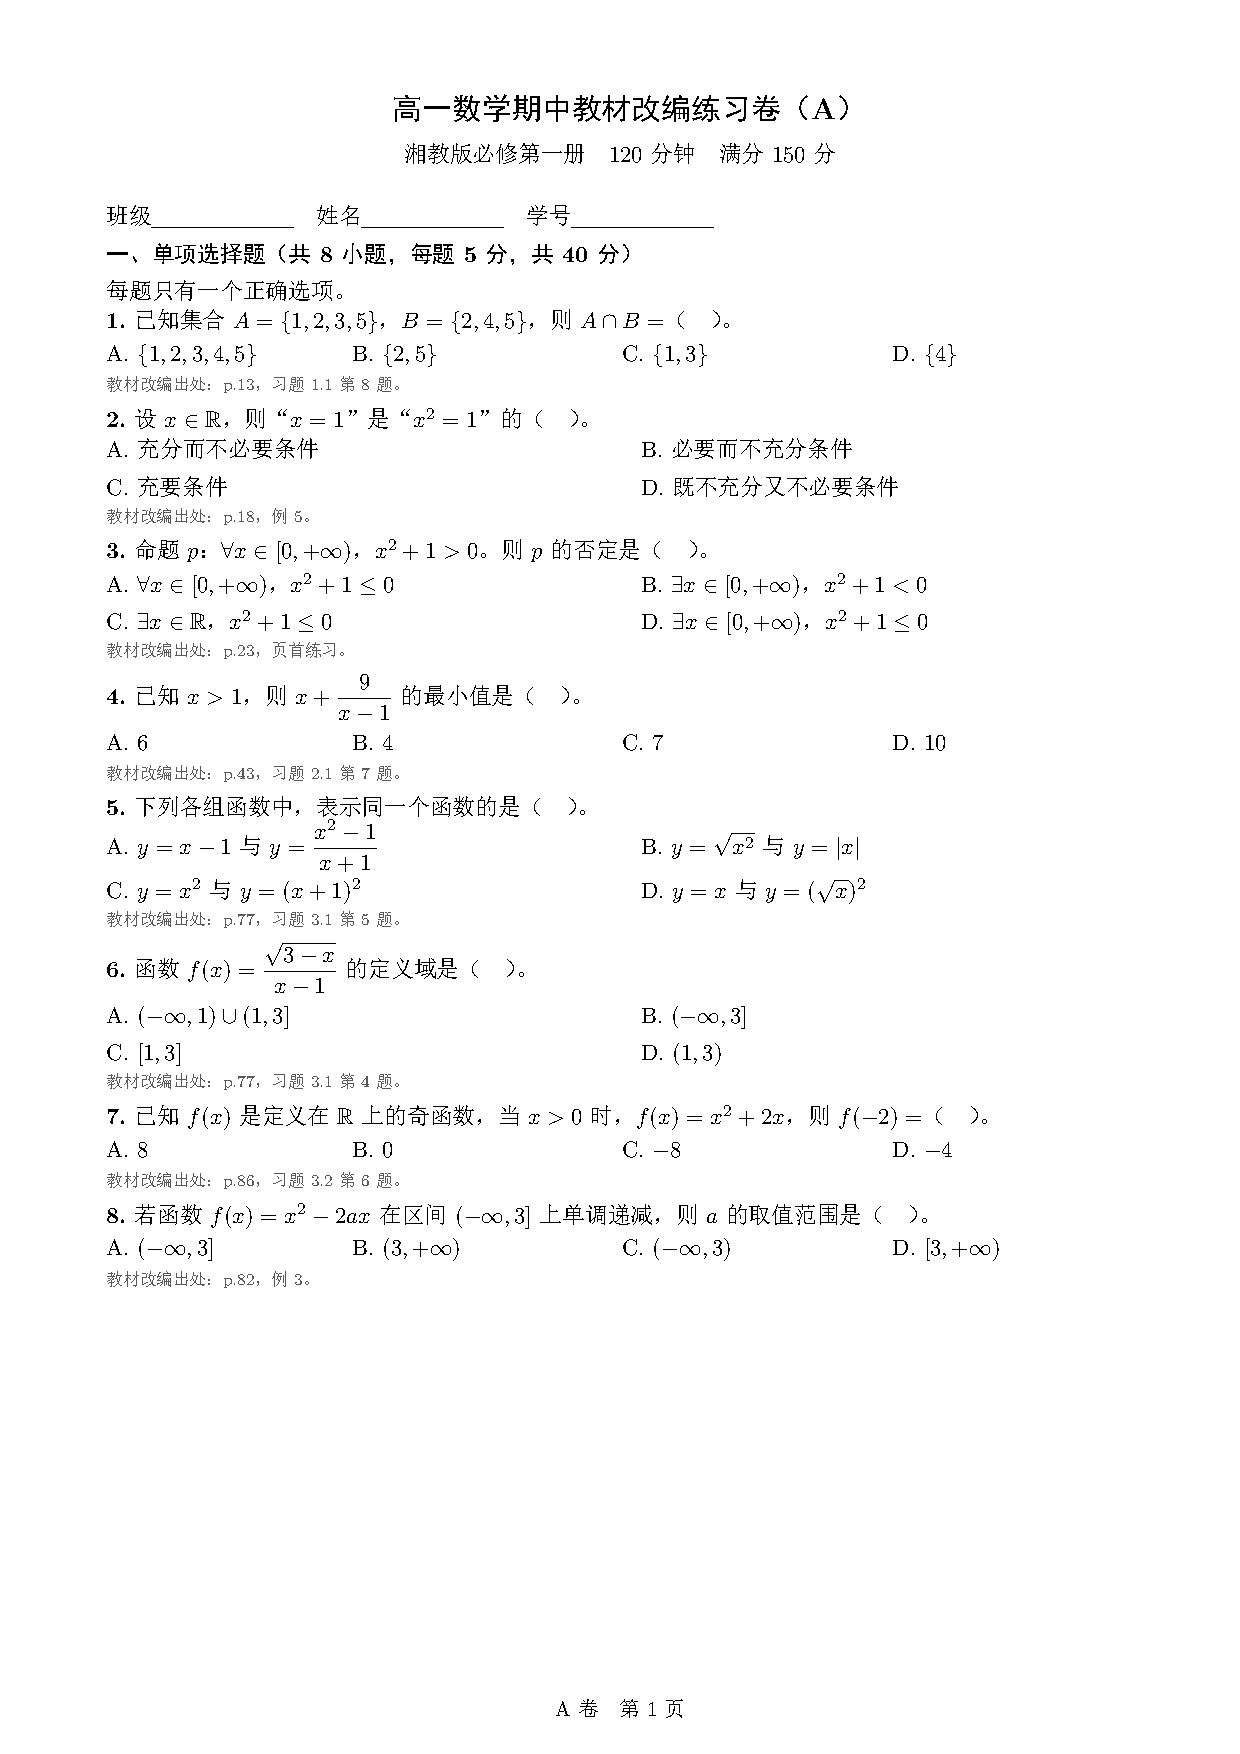
\includepdf[addtotoc={1,section,1,A卷学生卷,studentA}]{../A卷/A卷_学生卷.pdf}
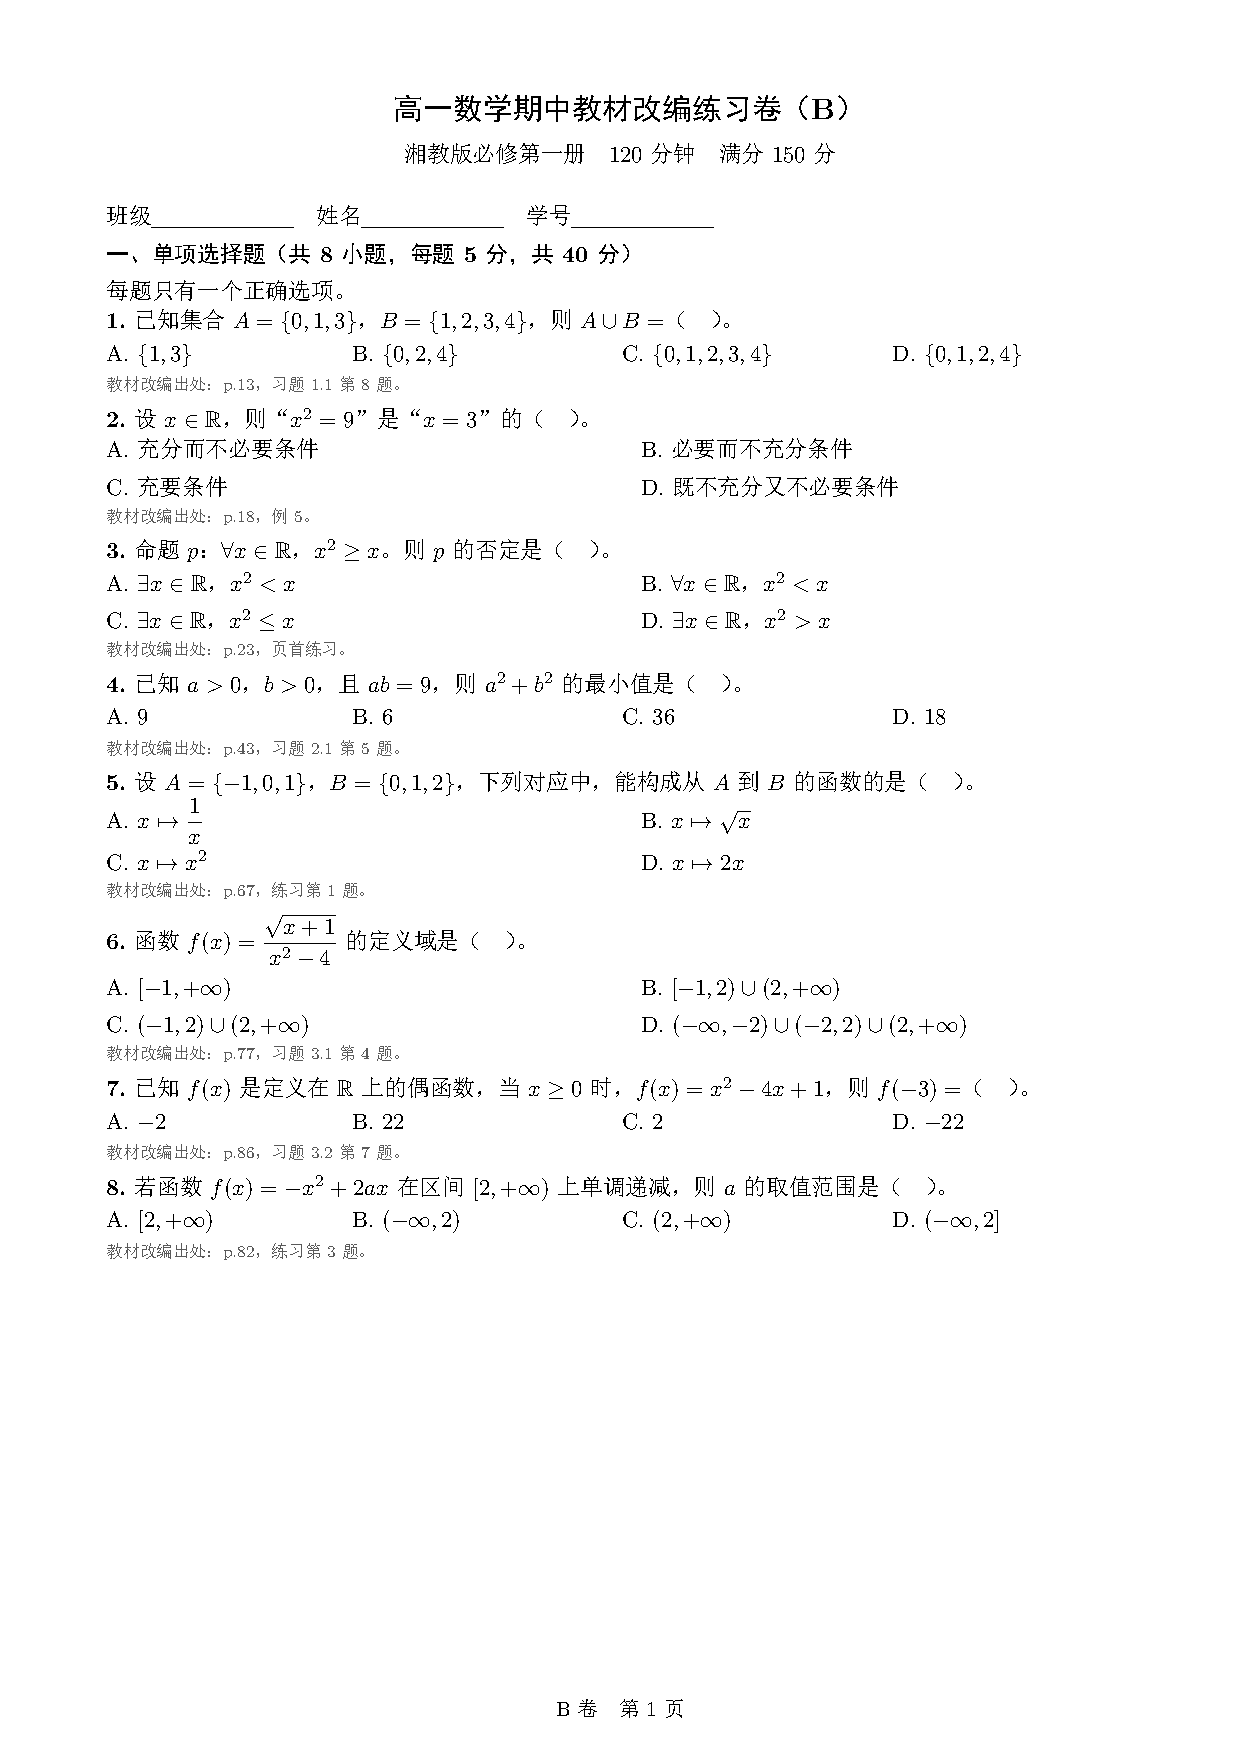
\includepdf[addtotoc={1,section,1,B卷学生卷,studentB}]{../B卷/B卷_学生卷.pdf}
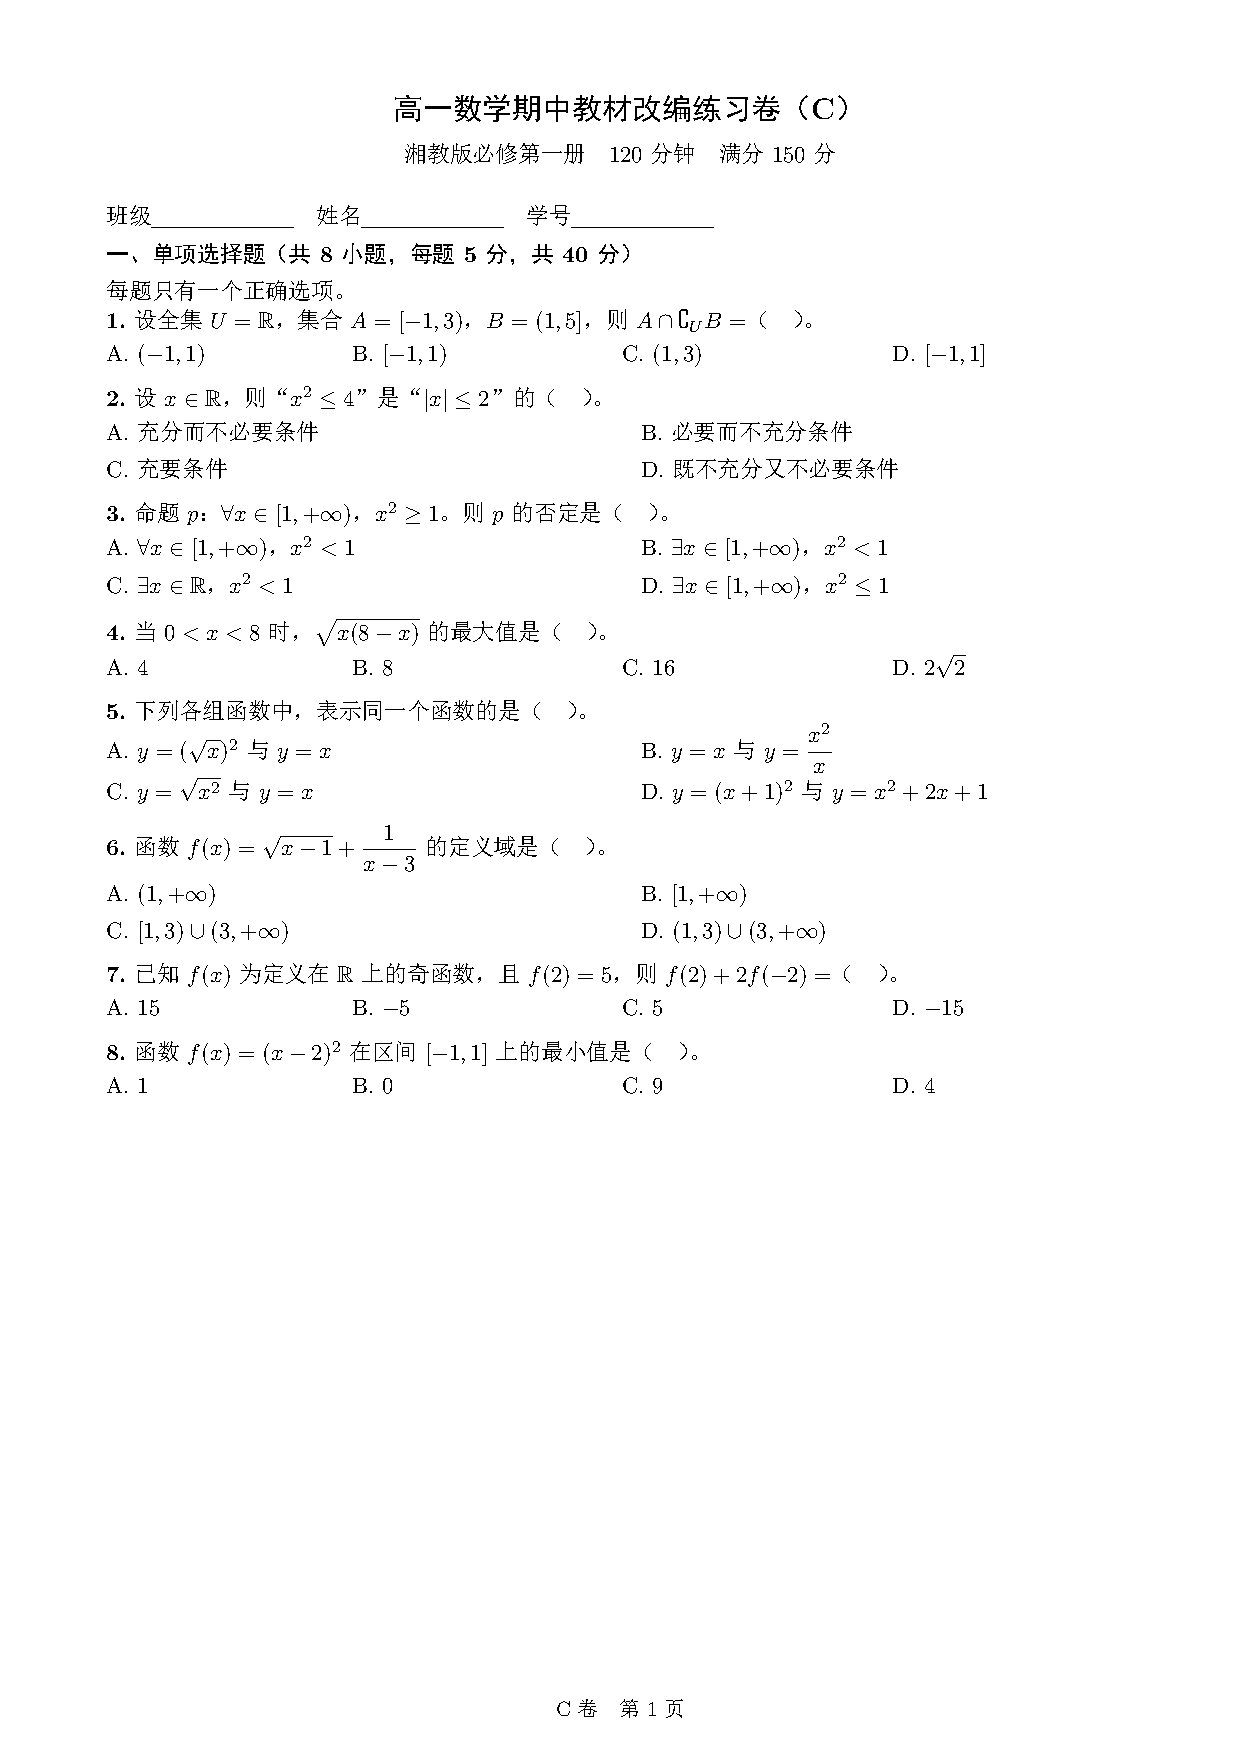
\includepdf[addtotoc={1,section,1,C卷学生卷,studentC}]{../C卷/C卷_学生卷.pdf}
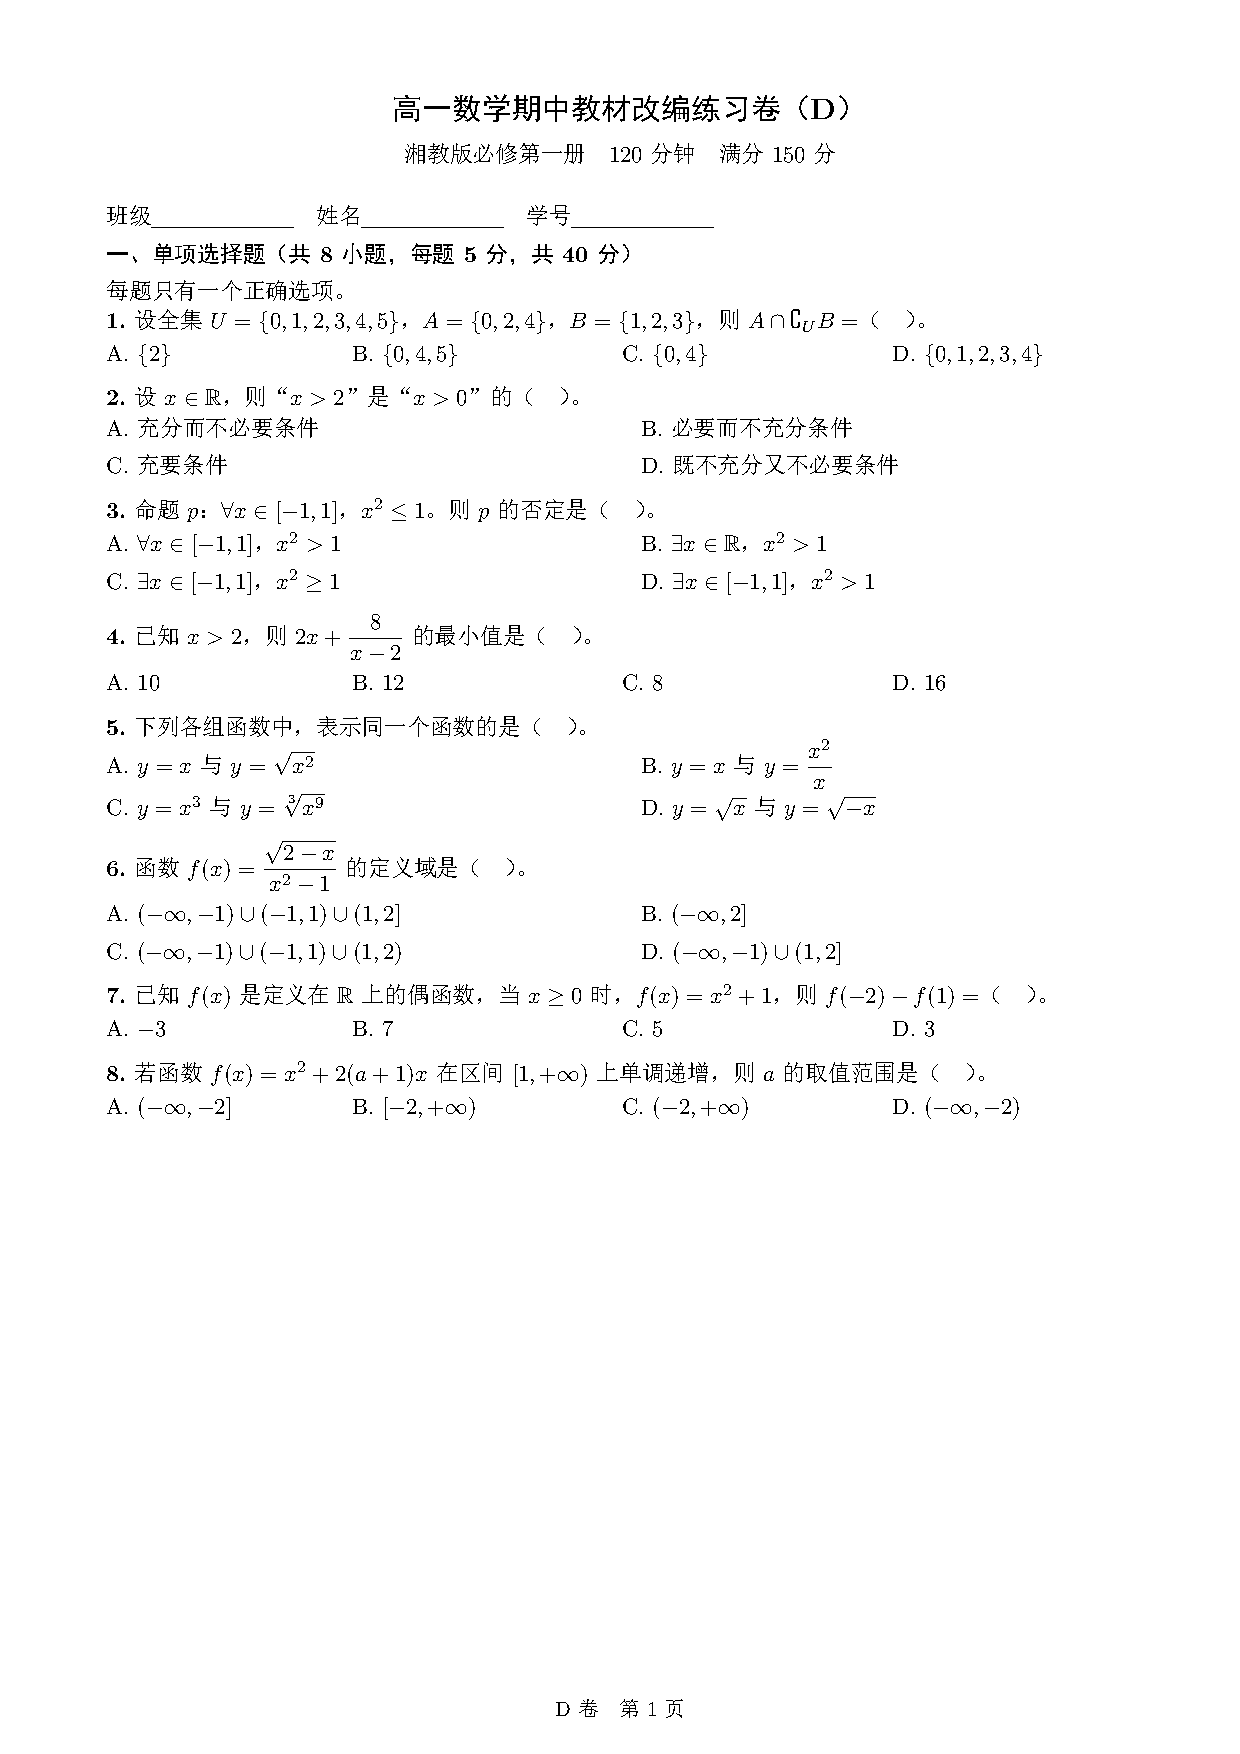
\includepdf[addtotoc={1,section,1,D卷学生卷,studentD}]{../D卷/D卷_学生卷.pdf}
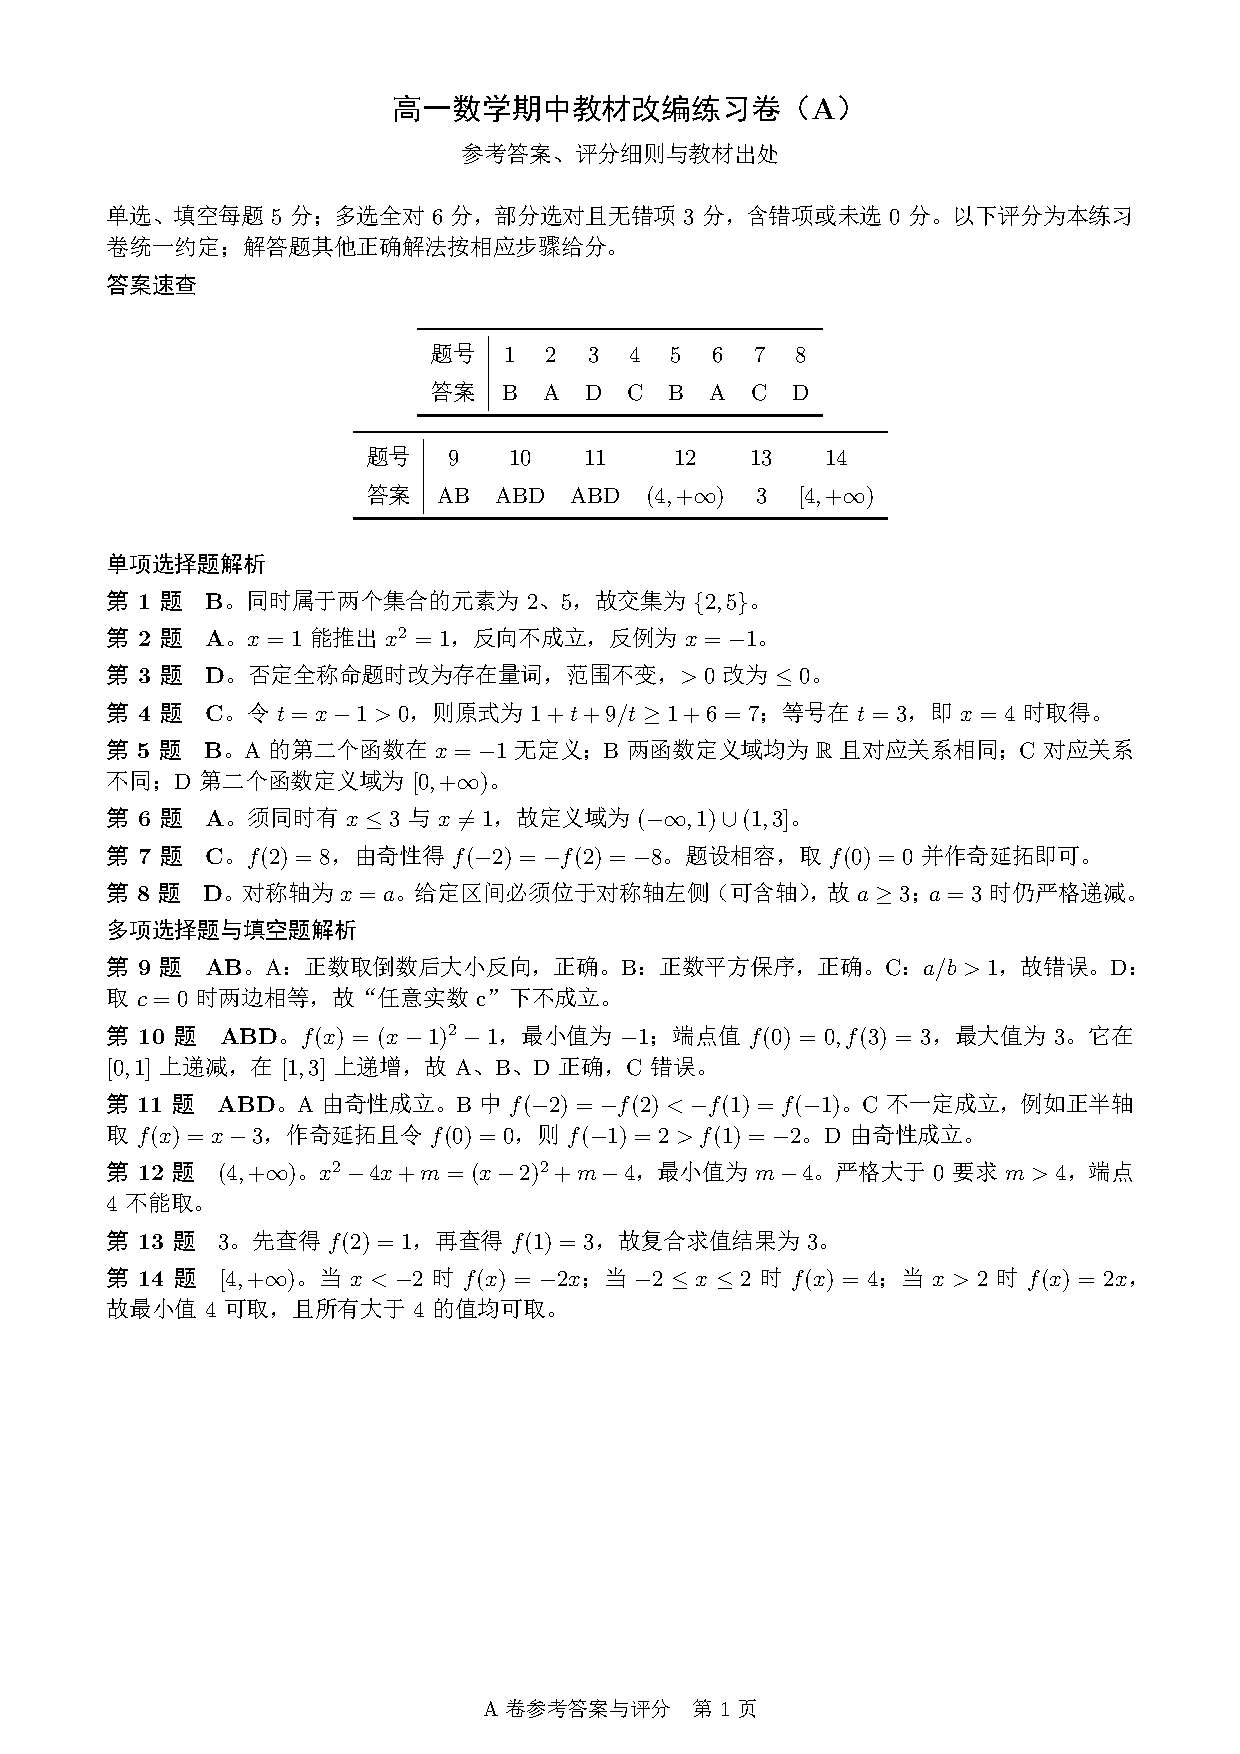
\includepdf[addtotoc={1,section,1,A卷参考答案与教材出处,teacherA}]{../A卷/A卷_教师版.pdf}
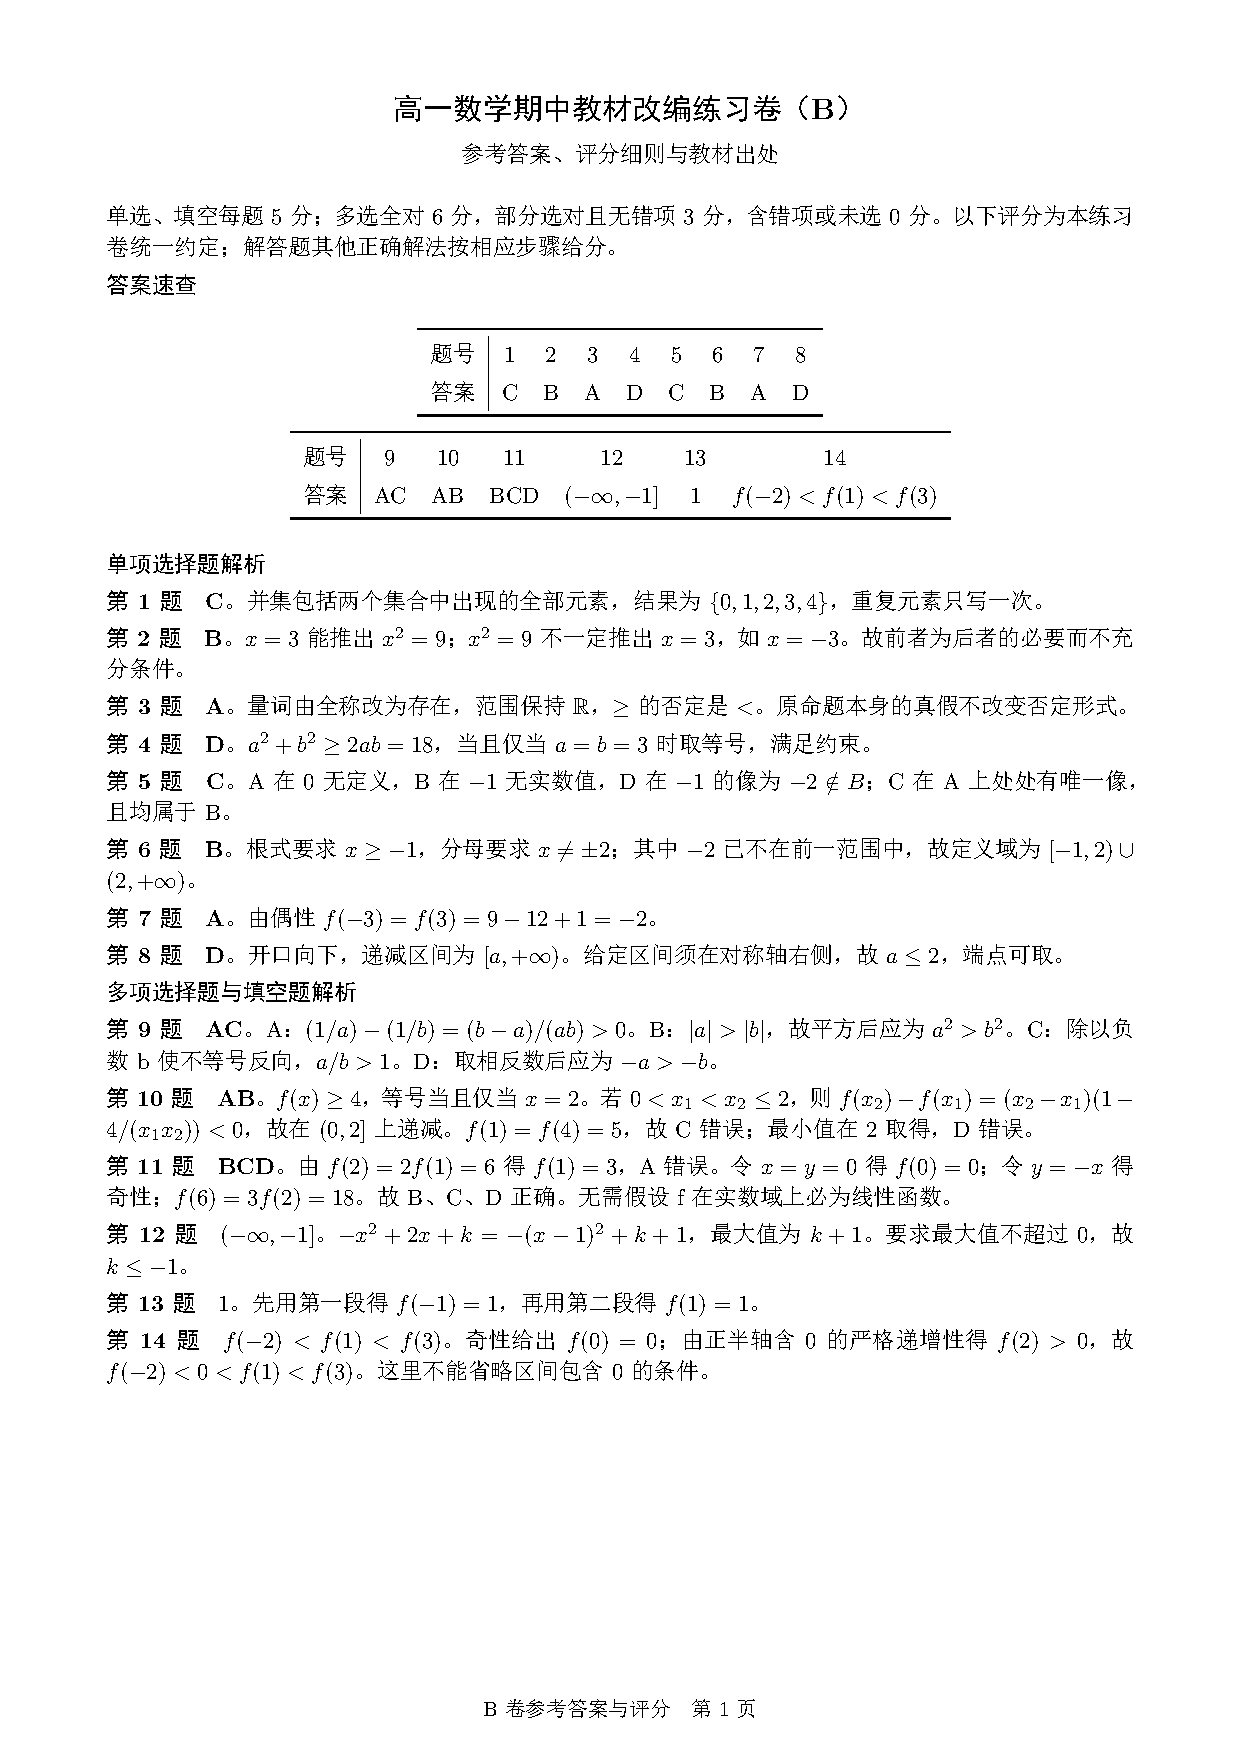
\includepdf[addtotoc={1,section,1,B卷参考答案与教材出处,teacherB}]{../B卷/B卷_教师版.pdf}
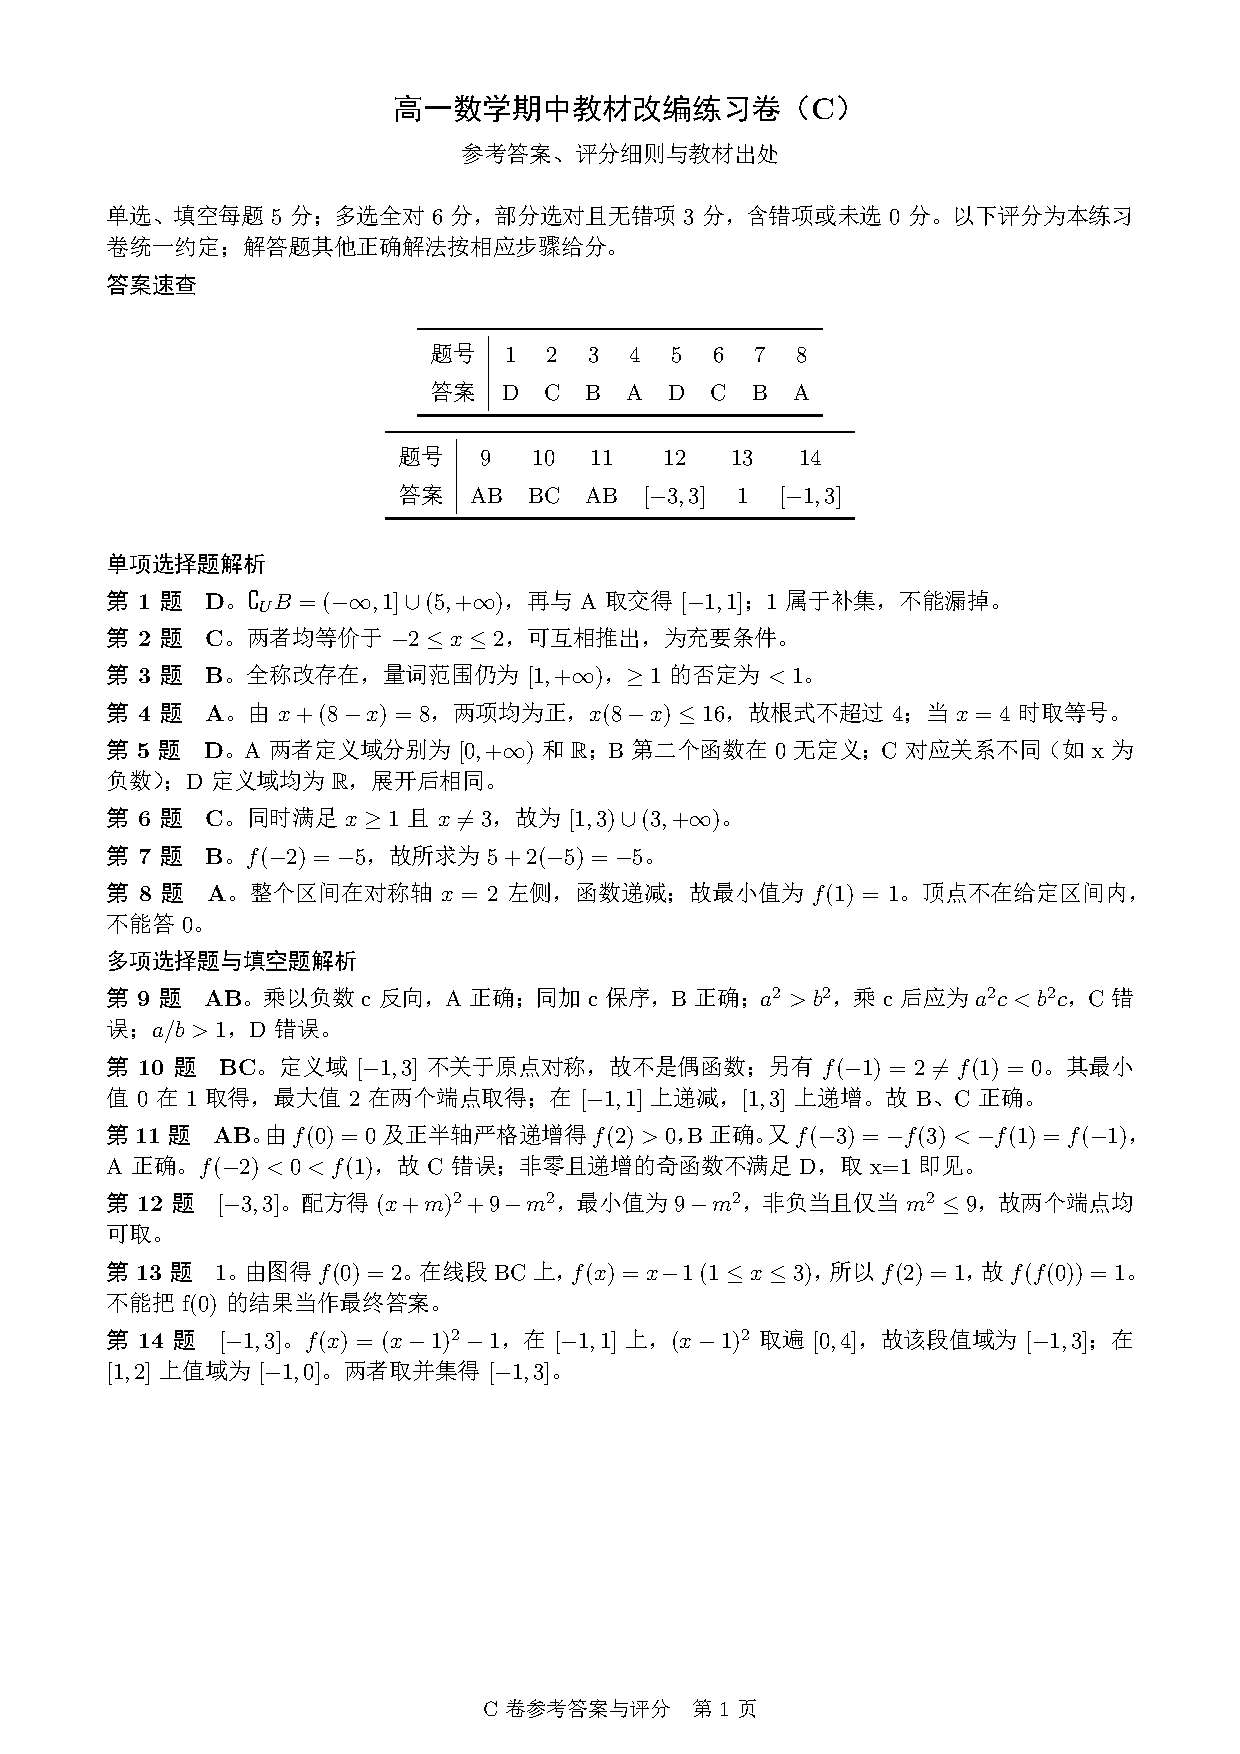
\includepdf[addtotoc={1,section,1,C卷参考答案与教材出处,teacherC}]{../C卷/C卷_教师版.pdf}
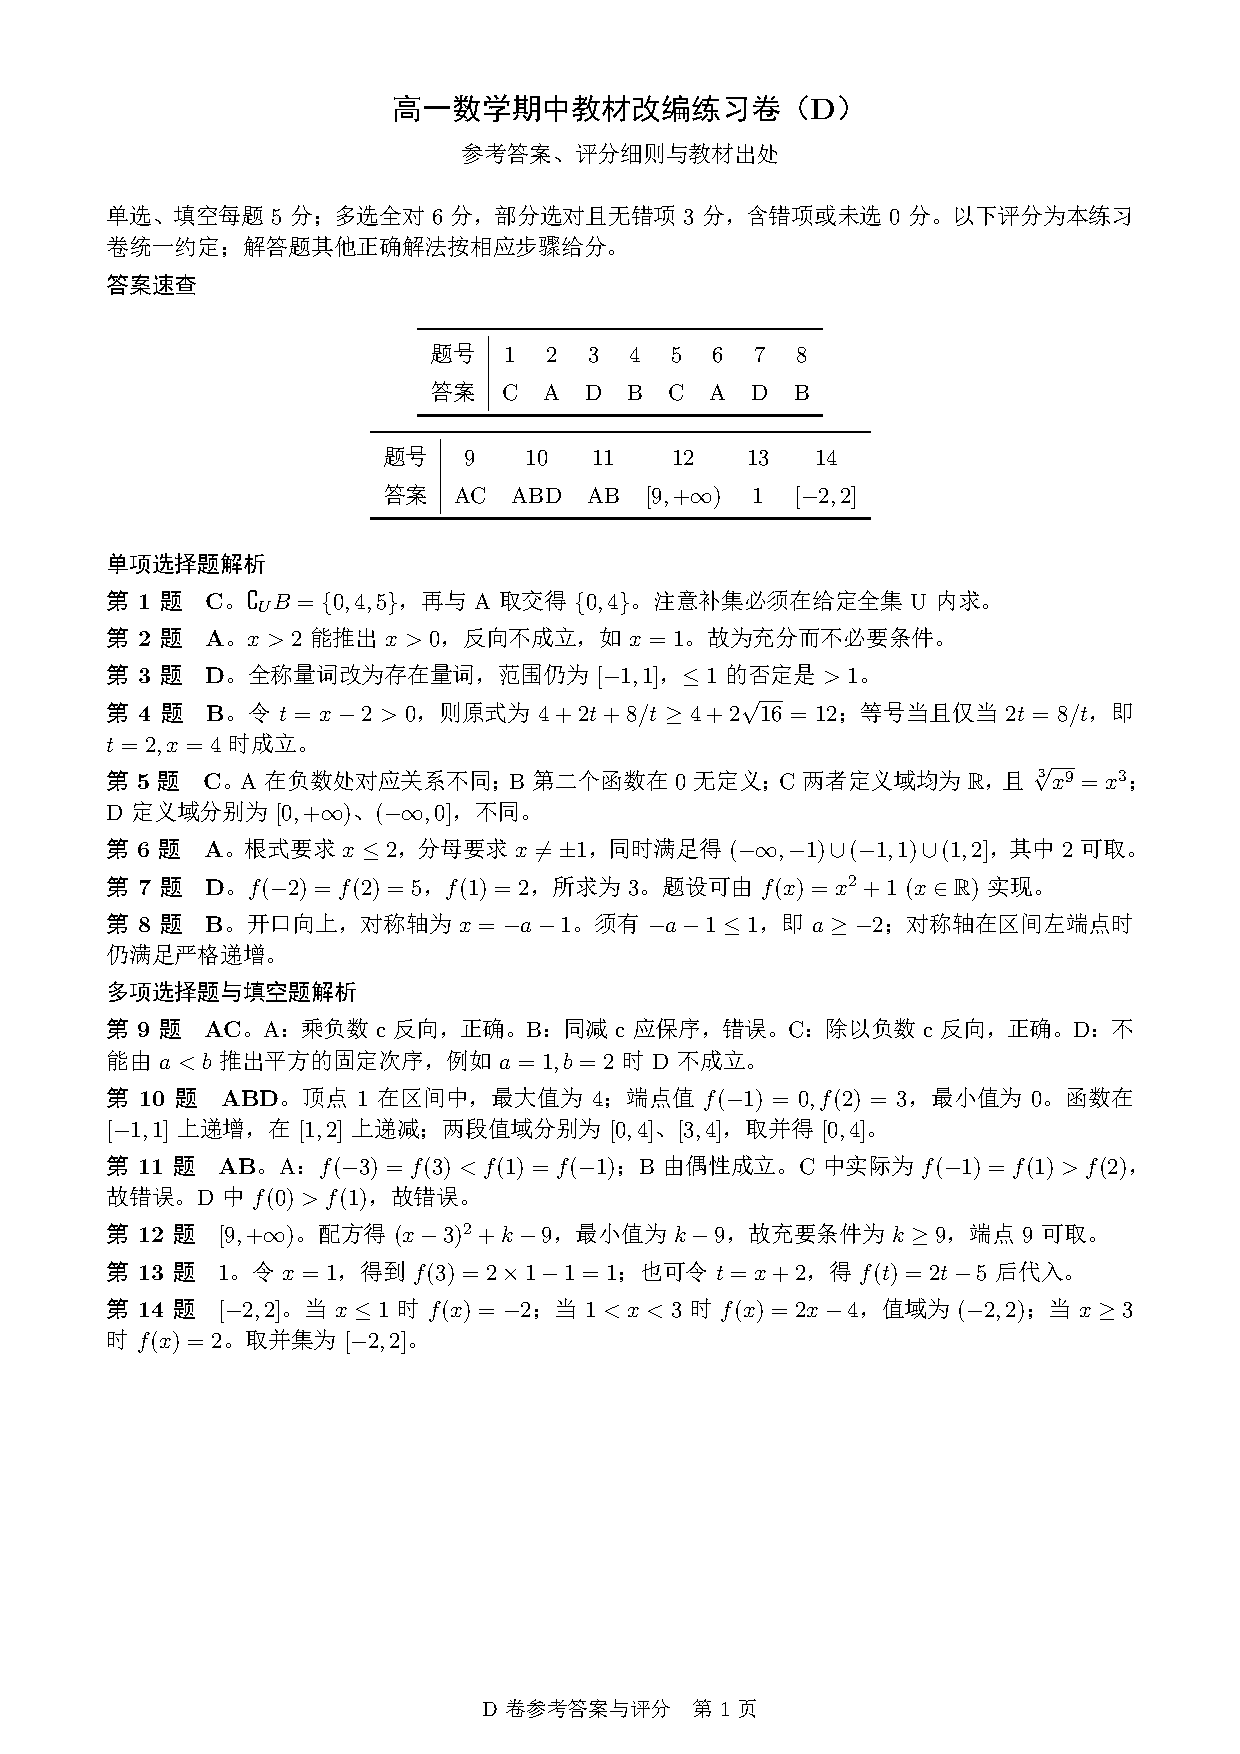
\includepdf[addtotoc={1,section,1,D卷参考答案与教材出处,teacherD}]{../D卷/D卷_教师版.pdf}
\end{document}
